\documentclass{sig-alternate}
\usepackage{color}
\usepackage[colorinlistoftodos]{todonotes}
\usepackage{amssymb}
\begin{document}
\todo[inline]{My paper is currently unfinished in spots where I am still figuring out how to explain a certain procedure. One thing I think would help me a lot is if you could comment on the general layout of the paper. Also, if there are spots that I should emphasize/Include more detail on or if there are spots that maybe should not be in the paper would also help me. Thank you for your time}
\conferenceinfo{UMM CSci Senior Seminar Conference, December 2014}{Morris, MN}

\title{Gait Recognition in Mobile Security}

\numberofauthors{1}

\author{
\alignauthor
Chase R. Ottomoeller\\
	\affaddr{Division of Science and Mathematics}\\
	\affaddr{University of Minnesota, Morris}\\
	\affaddr{Morris, Minnesota, USA 56267}\\
	\email{ottom005@morris.umn.edu}
}

\maketitle
%----------------------------------------------------------------------------------------------------------------------%
\begin{abstract}
This paper discusses a new form of mobile security not just emphasizing security, but also usability. Having a form of security of a mobile device that is unobtrusive can make that device easier and a less of a hassle to use. This paper will discuss using built in accelerometers in smart phones as way to collect biometric data. In this case the biometric data is a persons gait or walking pattern. This increases the security of the device by allowing the authentication to be not something you have or something you know, but something you are. There are two example that this paper will compare showing two forms of gait analysis. 
\end{abstract}

\keywords{mobile security, gait recognition, biometrics, accelerometer}
%----------------------------------------------------------------------------------------------------------------------%
\section{Introduction}
	As computational power in computers increases, the security risks grow higher for forms of authentication. One growing concern is security in mobile devices such as smart phones. Smart phones are also becoming increasingly more powerful, which results in more personal data being stored on the device. This means security for smart phones will become more important as time goes on. Currently security mainly consists of: pin, password, swipe lock, fingerprint. These forms are either something a person has(fingerprint) or something a person knows(password). They all also require a physical action to unlock the phone. A new form of mobile security involves a persons gait making it an unobtrusive form of security. This means that the built in accelerometer in the smart phone will analyze a persons walking pattern. If the phone tell that the current user should have access the phone will be unlocked, otherwise it will switch to the normal pin password. This will increase the security of the mobile device because the form of unlocking the device is now something you are and not something someone else can take form you. 
	This paper will analyze two different approaches for gait extraction/analysis.  Each paper uses a general format format of analyzing the data which includes: Preprocessing, Feature Extraction, and Gait Analysis. Preprocessing is the process of capturing biometric data. Feature extraction is taking the raw biometric data and locating distinctive characteristics. Gait Analysis is taking the feature extracted data,and running algorithm on it which will return a positive or negative result. Though each paper follows this general outline, they did each step in a different way.

%\begin{figure}
%\centering
%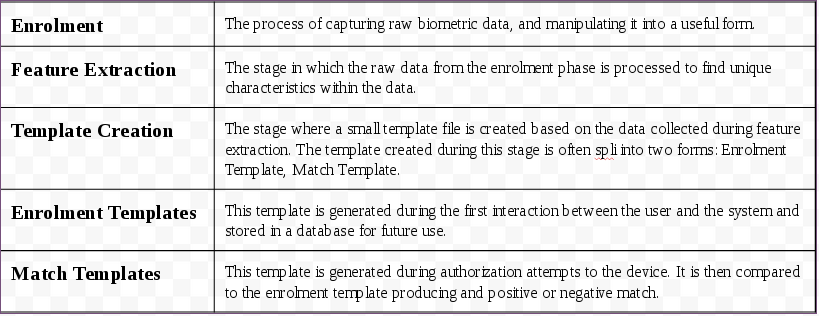
\psfig{file=chart3.png,width =3in}
%\caption{}
%\label{fig:Steps}
%\end{figure}

%I plan to use the following sources:
%\begin{itemize}
%\item one~\cite{Sujithra:2012}
%\item two~\cite{Muaaz:2013}
%\item three~\cite{Lu:2014}
%\end{itemize}
\todo[inline]{The introduction and background are similar and is being addressed.}
%----------------------------------------------------------------------------------------------------------------------%
\section{Background}
	As computers become more advanced, security becomes more important. This is especially relevant to mobile devices. More and more information is being stored on mobile devices, and securing that information is essential. Currently, the security for accessing mobile devices is based on something someone has (card or key) or something someone knows(pin or password). With these two current forms of security it is becoming easier to steal or compute the needed key to access the mobile device. 
		A new form of identificaton and verification is biometric based. Biometrics is used as a new form of security that provides unique identification to a mobile user. Now, instead of relying on a password of physical key, a person can gain access to their device by a physical trait specific to them. Some examples of biometric traits are: finger prints, facial features, eye, voice, hand, DNA, gait. In this paper I will focus on the gait recognition. The term gait refers to the walking pattern of a person. A persons walking pattern is cyclic in nature and may be composed of many gait cycles, where each gait cycle consists of at least two steps.~\cite{Sujithra:2012} 
			There are three types of biometric gait recognition: machine vision based, floor sensor based, and wearable sensor based. With mobile devices becoming more and more equipped with an array of sensors, the technique most suited for mobile devices is a wearable sensor based, using the mobiles devices built-in accelerometer. Data collected from the accelerometer will be processed in a set of operations later described. 
	In the next sections I will be comparing two approaches that use accelerometers from a mobile device such as a smart phone. The primary way in which these two approaches differ is the placement of the mobile device on the body. One approach has the smart phone in a fixed location on the waist. The other one has the smart phone in a more natural position on the body such as in a pocket. Though both papers use the general approach shown in figure 1 I will be simplifying them into three categories: Pre-Processing, Feature Extraction, and Gait Analysis. 
%----------------------------------------------------------------------------------------------------------------------%
\section{Preprocessing} 
Once data is gathered it needs to preprocesed into a usable form. In this case a usable form is modified data that has been separated into frames. A frame is equally separated parts of data for feature extraction and classification. With two experiments, separating the data into modified frames was done differently. The fixed phone method used a strict test case that was modified using Linear Interpolation and Zero Normalization. The unfixed phone method used Framing to separate the data into frames. These frames were then modified by a method known as Projection. In the following sections I will explain the fixed and unfixed methods as well as comparing them. 

\subsection{Interpolation and Zero Normalization }	
	With the phone on the waist in a fixed position, uniform sets of data called walks were used. In this case one walk is represented by walking a measured distance down a hallway. The experiment was done is such a way that one set of data contained two "walks", or in other words, one set of data was walking a hallway; Once down and once back. After extracted, this data is modified to further extract features. These modifications include linear interpolation and zero normalization. 
	
\subsubsection{Interpolation} 
	Once the walks are separated from the initial data, they have to be formed into equal intervals. This is done by applying \textit{Linear Interpolation}, which can reshape the data  into equal intervals. In order to not loose data during this change up-sampling is applied. Up-sampling avoids data loss by producing ``an approximation of the sequence that would have been obtained by sampling the signal at a higher rate''~\cite{wiki1:2014}. Once the data has been reshaped, the acceleration measurements have to be adjusted. 
	
\subsubsection{Zero Normalization}
	The PMD's accelerometer being used measures 3 axis(x, y, z). the only axis needed, and the only axis affected by gravity is the x axis. Since the acceleration for the y and z axis are not stable over time, and they are not affected by earth's gravity, the acceleration data for the y and z axis have to be \textit{zero normalized}. In other words the data for the y and z axis have to be set to zero. This is done by simply subtracting their total acceleration from there average acceleration. An overview of the stages explained above are shown in figure ~\ref{fig:firstStep}.

\begin{figure}
\centering
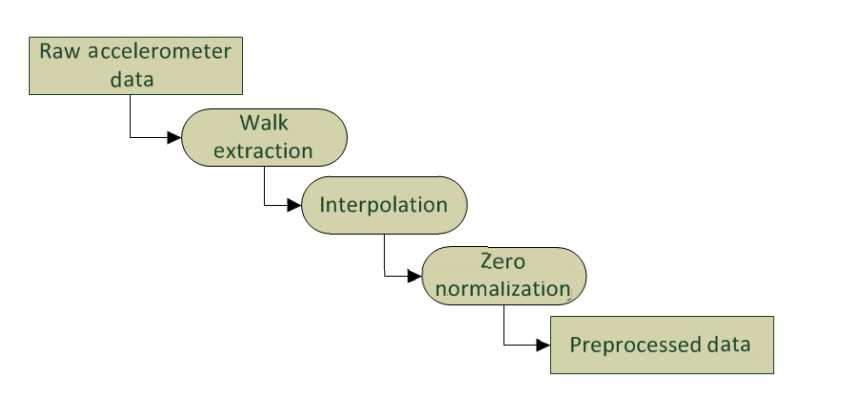
\psfig{file=chart1.png,width =3in}
\caption{Preprocessing Step}
\label{fig:firstStep}
\end{figure}
\todo[inline]{this figure is just a place holder till I make one that is nicer}

\subsection{Framing and Projection}
	The previous method used a phone in a fixed location. This method tries to expand on this with a phone in a unfixed location, such as a pocket. Also, this method is less strict. It does no use a set length, such as a hallway, to mark each walk. Instead this method uses a processes called \textit{Framing}. Once the data is segmented into frames it is then projected onto a global coordinate system through a process know as \textit{Projection}.
\subsubsection{Framing}
 In the framing step, sensor data was segmented into uniform frames for feature extraction and feature classification. The data in this case is split into 512 frames.
\subsubsection{Projection}
The accelerometer samples at 100 Hz allowing stationary frames to be dropped. Frames that involved non walking activities are taken into account using a process later described. Accounting for stationary movement is necessary because the case where someone stops walking is not useful data. Following the framing step comes the projection step. In the projection step each accelerometer sample is projected onto a global coordinate system. Each sample within a given frame contains an X, Y and Z coordinate. Each coordinate is then projected into a vertical and horizontal vector which represent the vertical and horizontal direction. Once each sample is projected the next step is to compute the direction of gravity. The reason for doing so is because unlike the previous example, this process doesn't assume a fixed location or orientation of the mobile device. They estimate the direction of gravity by low-passing accelerometer readings using a mean filter. This is done with the equation G = (mean(X), mean(Y ), mean(Z)) where X, Y and Z are the corresponding axes. This is useful for determining if the position of the mobile device has changed. If there is a significant change in G then the orientation of the device has changed. This means the corresponding frame will be dropped and the horizontal and vertical axes will be adjusted accordingly. 
\todo[inline]{replace the equation G = (mean(X), mean(Y), mean(Z)) with actual latex math notation}

%----------------------------------------------------------------------------------------------------------------------%

\section{Feature Extraction}
	\textit{Feature Extraction} is extracting a set of data from a given frame to detect patterns of walking. Another way to define feature extraction is the process of extracting gait cycles from the data.
\subsection{Modifying Cycles}
	Once the raw gait data is preprocessed then the next step is extracting the biometric gait cycles. The first step in extraction is estimating the cycle length. Estimating the cycle length is done by computing the minimum salience vector. A minimum salience vector contains one entry for each data point of the walk vector. This entry is the count of values between the current data value and the value in the walk vector. In order for each value of minimum salience to be considered a cycle, the start value has to be greater than the \textit{minimal peak height}, and has to have at least a distance of \textit{minimal peak distance}. In short a minimum salience vector which is greater than minimal peak height, and has at least the distance of minimal peak distance is considered a cycle start. Each minimal peak height and minimal peak distance are calculated differently based on the experiment. In this researched experiment the minimum peak height and the minimum peak distance was calculated by: \begin{displaymath}0.8 \times interpolation frequency \end{displaymath} \begin{displaymath}0.5 \times interpolation frequency \end{displaymath} 
	
An example of minimal salient vectors is shown in figure~\ref{fig:AccelChart} These minimum salient vectors are used for cycle detection. Note, minimums are not distinct enough for determining gait cycles so maximum salient vectors are used in the same way only to compute the maximum peaks. These maximums are used to find the exact minima. These peaks are used as cycle starts and stops. Once one cycle is located the next factor to look at is the cycle length. These cycle lengths are normalized, or set to equal length, by using linear interpolation. Once the cycles are normalized there still may be some outliers that need to be cleaned from the data. This is done by computing the pairwise distance using Dynamic Time Warping (DTW) ~\cite{Muaaz:2013} Dynamic time warping is ``an algorithm for measuring similarity between two temporal sequences which may vary in time or speed.''~\cite{wiki2:2014} Cycles that are removed are the ones with half the distance or less of the other cycles. Another overview of the completed stages so far is shown in figure~\ref{fig:SecondStep}.
\begin{figure*}
\centering
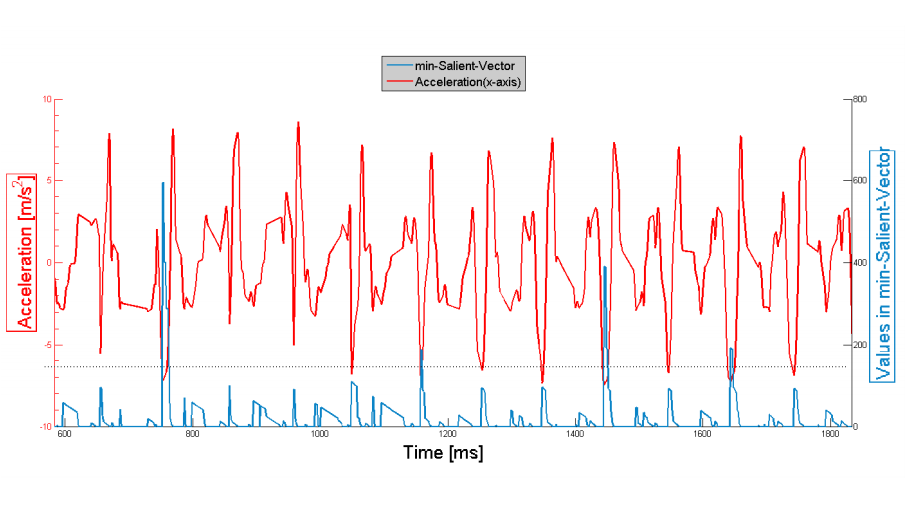
\psfig{file=svector.png,width =5.3in}
\caption{Minimum Salient Vectors}
\label{fig:AccelChart}
\end{figure*}

\begin{figure}
\centering
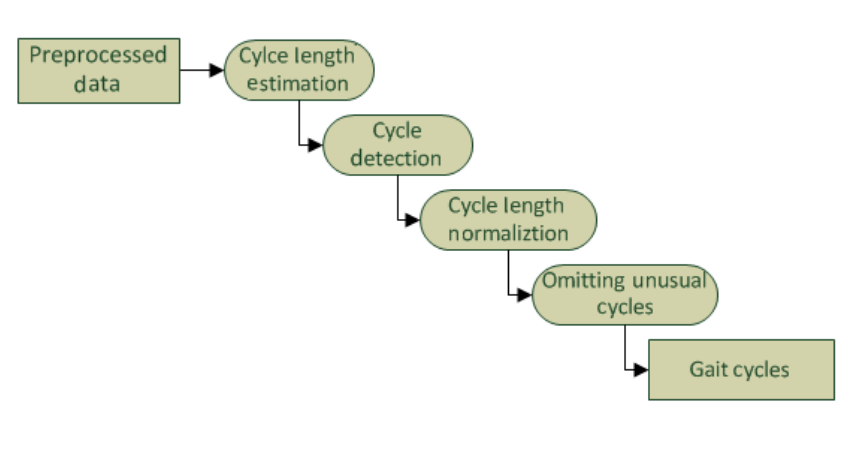
\psfig{file=chart2.png,width =3in}
\caption{Feature Extraction}
\label{fig:SecondStep}
\end{figure}

\begin{figure}
\centering
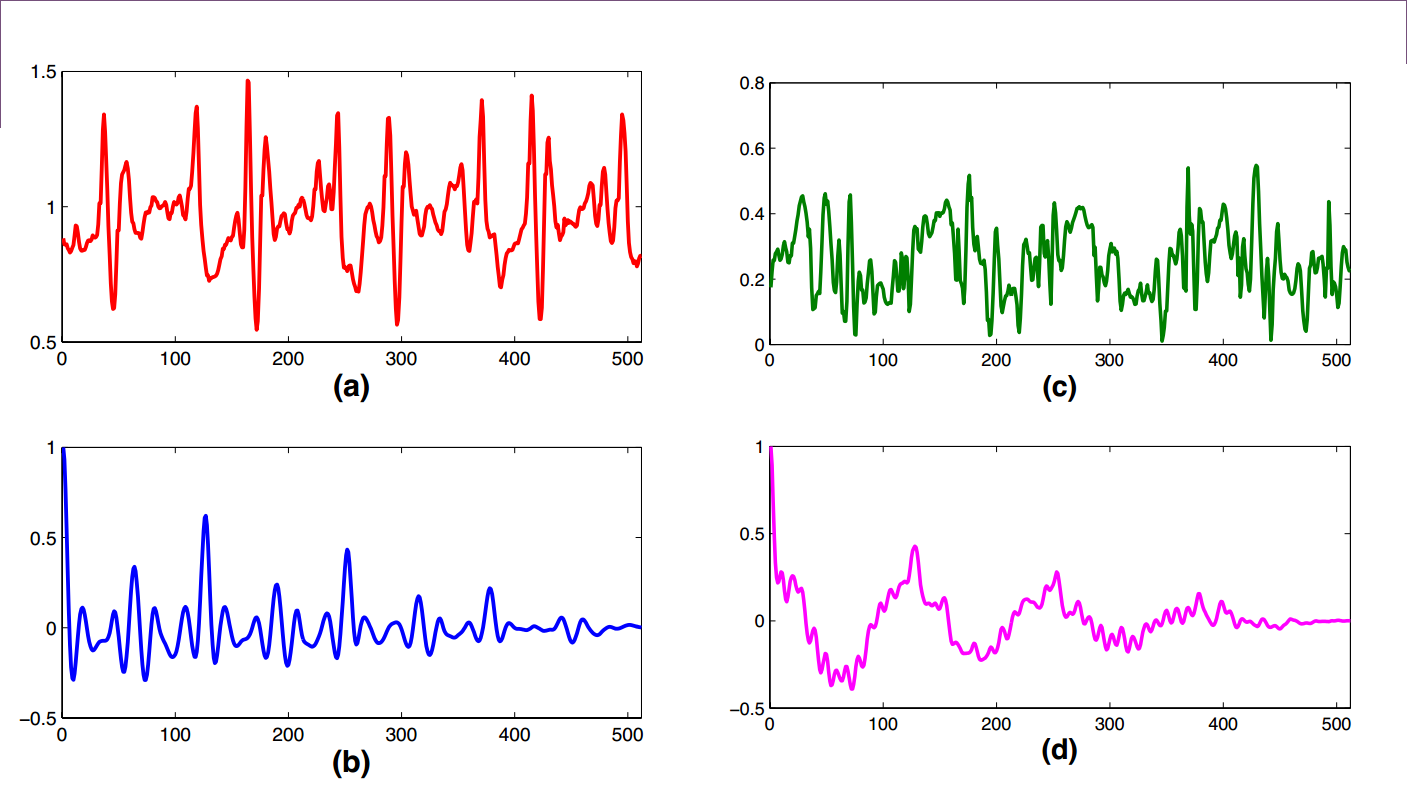
\psfig{file=abcd.png,width =3in}
\caption{(a) projected vertical component. (b) normalized autocorrelation of the vertical component. (c) projected horizontal component. (d) normalized autocorrelation of the horizontal component}
\label{fig:TD1}
\end{figure}

\begin{figure}
\centering
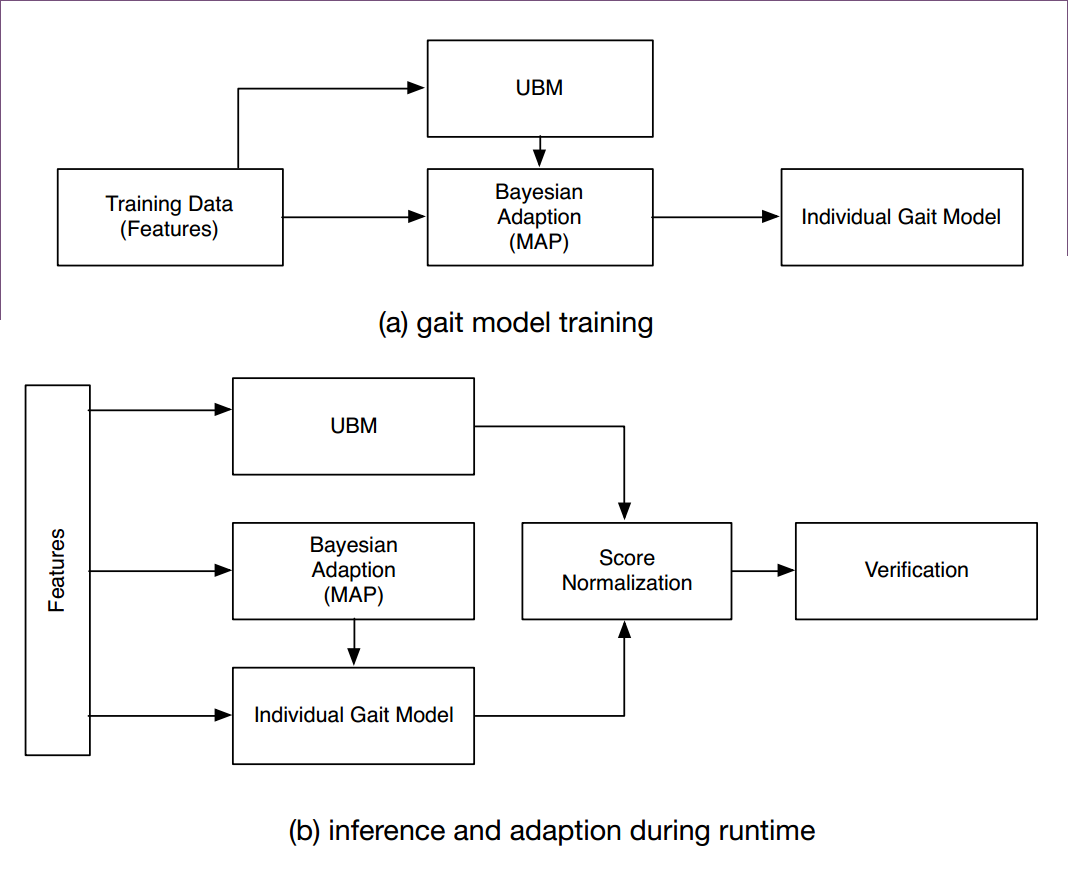
\psfig{file=FESP.png,width =3in}
\caption{Algorithm workflow for (a) generate user gait model by MAP adaptation (b) runtime inference and Individual model adaptation}
\label{fig:TD2}
\end{figure}

\subsection{Time-domain and Frequency-domain}
	A different form of extraction used by ~\cite{Lu:2014} uses a combination of time-domain, frequency-domain, and auto-correlation features. 
This example also did feature extraction in two stages: calculating the set of features for walking and calculating more precise gait features. 
The first stage of the feature extraction is used to tell whether or not the data represents walking data. This is done to rule out the times when the mobile device is not collecting the right data. For example if the mobile device was collecting data when it was in a car going down the road, that data shouldn't be used because it isn't gait data. This also holds true for collecting data on someone who is standing still. The data doesn't wouldn't represent the data needed for a biometric. Telling whether the data collected is of someone walking is done by collecting vertical and horizontal features to produce motion patters. Six time-domain features are used for both directions. These six feature are :mean, variance, skewness, kurtosis, energy, mean-crossing rate. All these features are based on spectrum analysis. In other words, doing ``different activities have different energy distributions over the frequency spectrum.''~\cite{Lu:2014} Walking can be measured around 1-2Hz while driving in a car will output a higher frequency band. Based on these frequency levels the data is put into one of three classes: walking, non-walking and motion(high frequency movement such as a in a vehicle or running).
The second feature extraction done once the data collected is determined to be that representing gait data. In this stage more relevant features are extracted for analysis. The first analysis to be done is the Compressed sub-band cepstral coefficients(CSCC). This is done in the following three steps. First, the energy spectrum is computed using the FFT spectrum. The Fast Fourier Transform(FFT) is an alogorithm that computes the Discrete Fourieer Transform(DFT) and its inverse. 
Second, the study maps the energy spectrum into 26 bands using triangular overlapping bands and sum up the energy in each band. Third, the processing takes the discrete cosine transform of the sub-band energy to form a 12-dimension vector representation. This in all summarizes the fundamental frequency of the movements and the higher frequency vibrations in the data.
\todo[inline]{This will need more in-depth explaining using ~\ref{fig:TD1} and ~\ref{fig:TD2}}

%----------------------------------------------------------------------------------------------------------------------%
\section{Gait Classification}
	This last step is taking the extracted features and verifying that those features match a stored set of features; the stored set of features being the users. The first paper uses Support Vector Machines(SVM's). The basic idea of SVM's is taking dimentional data and separating it into two classes. This involves the use of a Gaussian kernel defined in the following section. The second paper uses a Gaussian Mixture Model - Universal Background Model(GMM-UBM) framework to verify a individuals gait. The basic idea with this technique is with scoring. Verification of a users identity is done by comparing the likelihood score from a users gait pattern to the universal back ground model. The universal back ground model represents human gait patterns in general.




\begin{figure}
\centering
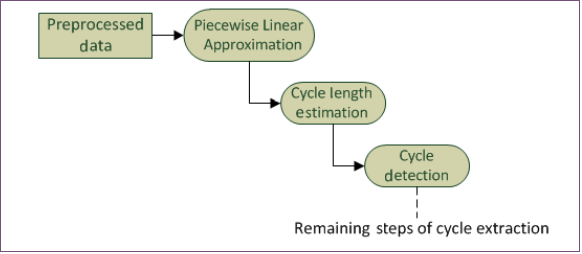
\psfig{file=PreprocessedData.png,width =3in}
\caption{Gait cycle extraction steps with Piecewise Linear Approximation(PLA)}
\label{fig:AddedStep}
\end{figure}

\subsection{Template-based classification}
	The template-based classification uses the same approach for gait extraction as shown in~\ref{fig:SecondStep} with one extra step added show in \~ref{fig:AddedStep}. Before the Cycle Length Estimation module is Piecewise Linear Approximation(PLA). A Piecewise Linear Function(PLF) is used to for the PLA. A PLF is a function composed of straight-line sections connecting points on a graph. So, a PLA is an approximation of a function connecting significant points on the curve with straight-line sections. The approach used to produce the PLA representations is the\todo[inline]{define swab}
Sliding Window And Bottom-up(SWAB). Once the unusual cycles are omitted, the best cycle is picked. The best cycle is determined by having the lowest DTW 
\todo[inline]{make sure DTW is explained somewheredistance.} 
%\todo[inline]{make sure that best cycles are reference cycles}
One the best cycle is foundA the remaining cycles are called probe cycles. These two sets of cycles are compared using the DTW distance to compute the genuine and impostor class. The DTW of each cycle is computed and majority voting takes place. If 50\% or more of the comparisons returns and accept then the cycle in a genuine, otherwise it's rejected as an imposter. \todo[inline]{figure out what the EER is}





\begin{figure}
\centering
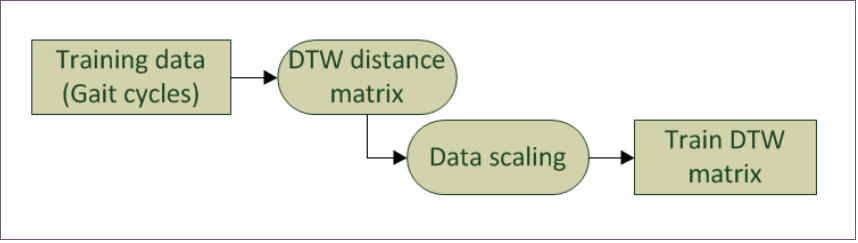
\psfig{file=TrainingData.png,width =3in}
\caption{Preparing data for SVM)}
\label{fig:TrainingData}
\end{figure}

\subsection{Machine learning based classification}
	SVM is another way that this paper classified gait data. SVMs are often used for biometric recognition, where imposter and genuine data have been determined. In simple terms a SVM finds a hyperplane that linearly separates \begin{math}\mathcal{D} \end{math} dimensional data into two classes. The dimensional data has to be linearly separable for SVM to work. Since the gait data isn't linearly separable, a ``kernel induced feature space''~\cite{Muaaz:2013} is introduced in SVM. A kernel function maps non linearly separable data to a high dimensional space. One mapped to a high dimensional space the data is lenearly separable and therefore can be used in the SVM. This means that depending on the kernel function you use, the better classification accuracy it will produce. a kernel function is defined as:

\begin{displaymath}
K : X \times X \rightarrow \mathbb{R}, \forall \{x,z\} \in X
\label{eq:KF1} 
\end{displaymath}

\begin{displaymath}
K(x,z)=< \phi (x).\phi(z) > 
\label{eq:KF2}
\end{displaymath}

Another more commonly used kernel function is the Gaussian kernel, which uses the Euclidean distance. Since the Euclidean distance restricts to only using fixed length cycles, using the DTW distance gets rid of this restriction. Two different approaches now can be used to classify gait cycles:Pre-computed data matrix, Pre-computed kernel. ~\ref{fig:TrainingData}

\todo[inline]{These two sections are being expanded with far more detail}
\subsubsection{Pre-computed data matrix}
	Gait cycles are represented by the DTW distance. This is the distance between two gait cycles. The benefit of the DTW distance is that different length gait cycles can be found. A DTW matrix is then computed from the sample and the other remaining gait cycles. This matrix is needed as an input for the SVM. 
\subsubsection{Pre-computed Kernel}
Using GDTW kernel ~\ref{eq:KF3} as the kernel matrix also allows to classify the gait data.

\begin{displaymath}
K(x,z)=exp(-\gamma \parallel DTW(x,z) \parallel ^2)
\label{eq:KF3}
\end{displaymath}

\subsection{Paper 2 Gait Classification}
%----------------------------------------------------------------------------------------------------------------------%
\section{Experiment Results}
\todo[inline]{compare and contrast the results each method yielded}
\subsubsection{Paper 1(title place holder)}
\subsubsection{Paper 2(title place holder)}

\begin{figure}
\centering
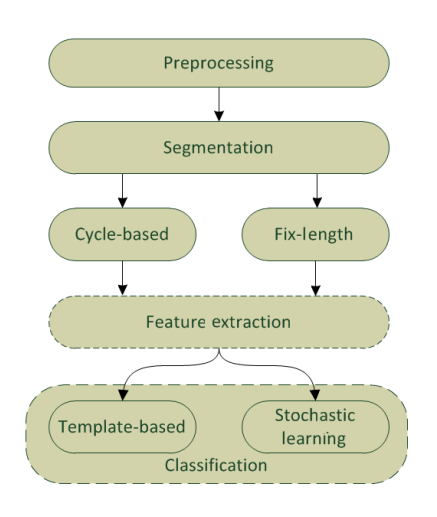
\psfig{file=sumary1.png,height =2.5in, width =2in}
\caption{Algorithm Overview}
\label{fig:Paper1Summary}
\end{figure}

\begin{figure*}
\centering
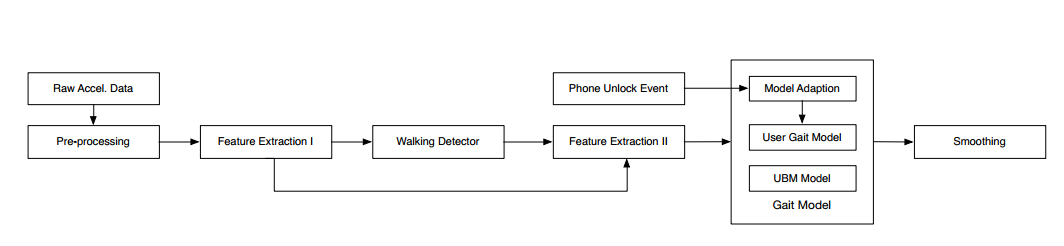
\psfig{file=sumary2.png,width =5.3in}
\caption{Algorithm Overview}
\label{fig:Paper2Summary}
\end{figure*}
%----------------------------------------------------------------------------------------------------------------------%
\section{Conclusion}
\todo[inline]{Compare how both methods were set up and briefly go over the outcomes using figures ~\ref{fig:Paper1Summary} ~\ref{fig:Paper2Summary} of each method again. Explain future work that will be done and how each method may be improved in the future}
I have compared two forms of using built gait as a form of mobile security. One experiment used a fixed location for the device while the other used multiple locations. Both use different methods of extracting the gait data as well as well as analyzing the data, but each method works. Both of these experiments are not perfect yet but they both show promise in using walking patterns as a form of mobile security. With more sampling/testing as well as improving efficiency with algorithms will improve these mobile security methods and show potential to become implemented in a large scale.
%----------------------------------------------------------------------------------------------------------------------%

\section{Acknowledgments}
\todo[inline]{right out a proper acknowledgement paying close attention to correct spelling of names}
% The following two commands are all you need to
% produce the bibliography for the citations in your paper.
\bibliographystyle{abbrv}
% annotated_bibliography.bib is the name of the BibTex file containing 
% all the bibliography entries for this example. Note that you *don't* include the .bib ending
% in the \bibliography command.
%----------------------------------------------------------------------------------------------------------------------%
\bibliography{paper}  

% You must have a ".bib" file and remember to run:
%     pdflatex bibtex pdflatex pdflatex
% in order to see all the citation references correctly.

\end{document}



